\chapter{Systems and Implementations}
\label{chpt:sytems}

\section{Aurox Clarity System}
\label{sec:aurox}

Confocal laser scanning microscopy (CLSM) is, traditionally, a point-scanning microscopy technique pioneered with the objective of discarding the scattered illumination light and the out-of-focus excited fluorescence when imaging biological samples.\cite{minsky1988memoir} Discarding the out-of-focus light yields images with high contrast and good optical sectioning.\cite{nwaneshiudu2012introduction} The original Minsky design struggled with a low-frame rate. Advances in technology have led to improved scanning speeds and therefore improved image frame rates which, for modern CLSM set-ups, is 0.1-1 fps.\cite{xiao1988real,schermelleh2010guide}. For many dynamic biological processes this is still insufficient, which lead to the development of (among other things) the Nipkow-Petran spinning disk setup which allows for video rate confocal imaging.\cite{egger1967new,fuseler2018types,tsien1995video} Hence, spinning disk confocal microscopes are frequently used for imaging live biological processes.

The Nipkow-Petran design does have disadvantage in that it discards $\sim99\%$ of both excitation and emission light in order to achieve good optical sectioning and \textit{xy}-resolution.\cite{kino1995intermediate} This can lead to poor signal-to-noise ratio (SNR) in fluorescence imaging if sufficiently strong fluorophores aren't used.\cite{semwogerere2005confocal} Fortunately, another design exists called a Correlation Disk which uses light emitting diodes (LEDs) as the illumination light source in conjunction with a patterned disk which is placed in a location shared by both the excitation and emission beam paths.\cite{juskaitis1996efficient,wilson1996confocal,neil1997method} The Aurox Clarity module employs just such an approach to achieve real-time confocal imaging with a significantly increased light budget ($25\%-50\%$ compared to $\sim1\%$). This approach relies on good correlation between the grid patterns present in both the excitation and emission paths, which is degraded by optical aberrations.\cite{hussain2020sensorless} Therefore, the Aurox Clarity System incorporates both the Aurox Clarity module for fast, laser-free confocal imaging and a deformable mirror (DM) for aberration correction.

\subsection{Aurox Clarity System Optical Set-up}
\label{subsec:aurox_optics}

Figure~\ref{fig:aurox_beam_path} shows the complete optical schematic of the Aurox Clarity system. Its base is a iX71 Olympus microscope body with a AMEP4694 $60\times$, 1.4 NA oil objective and P-736.ZR1S PI-nano Z Microscope Scanner piezo Z-stage. Ordinarily, the Clarity module would be attached to the side port of the microscope body. The Mirao52e 52-actuator DM must be placed in a plane conjugate to the back pupil plane in order to correct for the aberrations. To achieve this, the Clarity module is separated from the main microscopy body by a 4f, unity magnification telescope. The 4f telescope re-images the image plane close to the side port onto input port of the Clarity module and the DM is placed at the intermediate pupil plane. The Mirao52e DM was calibrated using a separate set-up not shown which uses a technique based on deflectometry.\cite{trumper2016instantaneous,huang2017close} A Photometrics PrimeBSI camera is attached to the Camera port of the Aurox Clarity module. A pE-300 Ultra CoolLED is attached to the Illumination light input port.

\begin{figure}[h]
	\begin{subfigure}{0.48\textwidth}
		\centering
		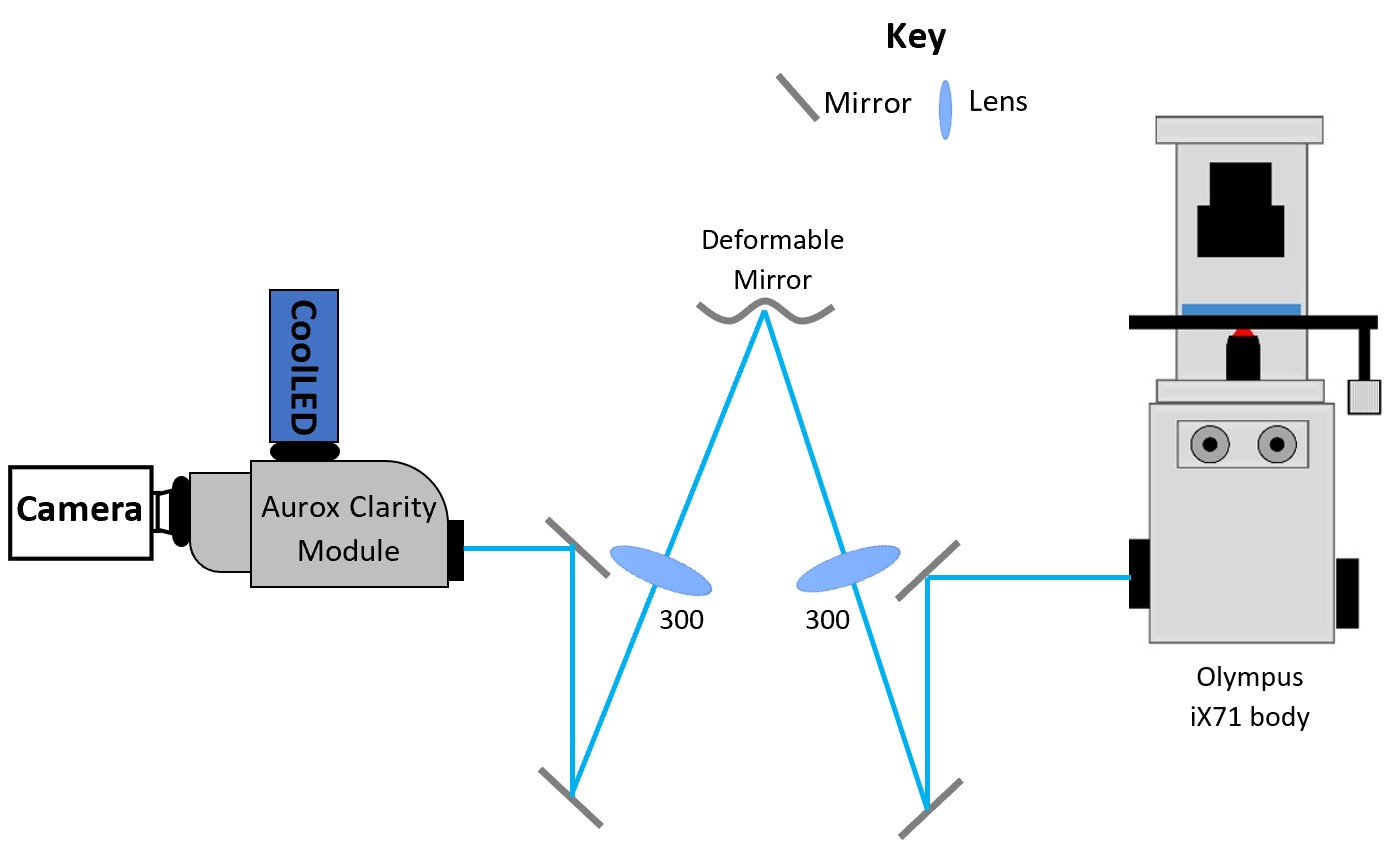
\includegraphics[width=\linewidth]{images/Aurox_beam_path.jpg}
		\caption{}
		\label{fig:aurox_beam_path}
	\end{subfigure}
	\begin{subfigure}{0.48\textwidth}
		\centering
		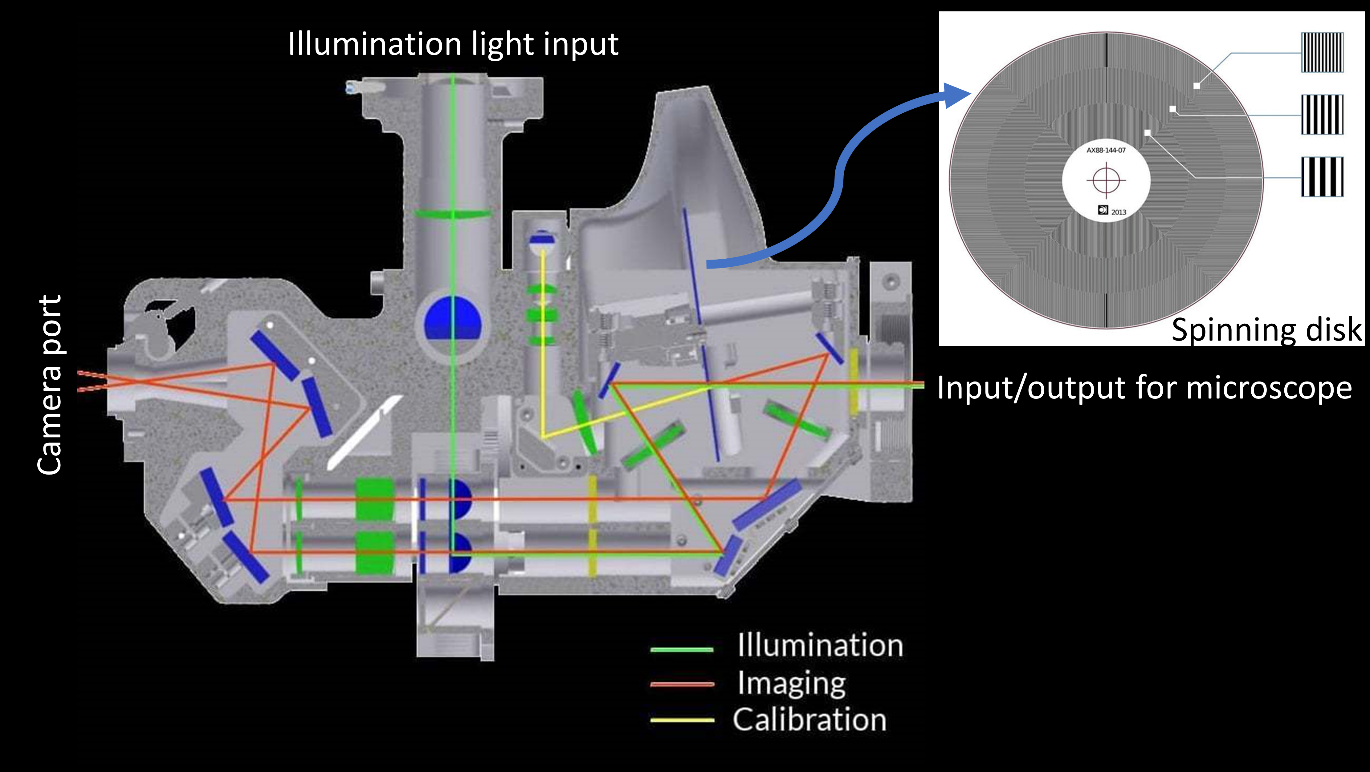
\includegraphics[width=\linewidth]{images/aurox_clarity_internal.png}
		\caption{}
		\label{fig:aurox_clarity_internal}
	\end{subfigure}
	\caption{Aurox system beam path layout (a) The complete imaging beam path for the Aurox Clarity System. The excitation and emission beam paths are identical up to the Aurox Clarity module (b) The internal beam paths for the Aurox Clarity module (Modified with permission from Aurox Ltd., Copyright Aurox Ltd.)}
	\label{fig:aurox_system}
\end{figure}

The excitation and emission beam paths are identical from the Input/output for microscope port to the focal plane of the objective. The differing beam paths for the excitation and emission light within the Clarity module are shown in Figure~\ref{fig:aurox_clarity_internal}. The excitation light impinges on the spinning disk and is either transmitted by the disk or discarded. The emission light impinges on the spinning disk in the opposite direction. The emission light from the focal plane of the objective is transmitted by the disk and is directed to one half of the PrimeBSI camera chip. The rest of the emission light is reflected off the disk and directed to the opposite half of the PrimeBSI camera chip. The Calibration light source generated within the Clarity module is used to align the two halves of the PrimeBSI camera chip to one another. A set of dichroic filter cubes are used to select both the excitation and emission wavelengths. There are four available dichroic filter cubes which can be selected:

\begin{enumerate}
	\item Dichroic filter 1: Excitation 466nm/FWHM 40nm, Emission 525nm /FWHM 45nm
	\item Dichroic filter 2: Excitation 554nm /FWHM 23nm, Emission 609nm /FWHM 54nm
	\item Dichroic filter 3: Excitation 578nm /FWHM 21nm, Emission 641nm /FWHM 75nm
	\item Dichroic filter 4: Excitation 392nm /FWHM 23nm, Emission 447nm /FWHM 60nm  
\end{enumerate}

\section{DeepSIM}
\label{sec:DeepSIM}

3D structured illumination microscopy (3D-SIM) is a super-resolution microscopy technique which is well suited to imaging live biological samples due to the relatively few images required to reconstruct a super-resolution image, millisecond temporal resolution, medium energy load, true multi-colour imaging and fast volume acquisition.\cite{schermelleh2010guide,schermelleh2019super} 
However, to date this application has not been extensively exploited for all live sample preparations, namely those requiring dissection and bathing, and those requiring dynamic sample manipulation such as electrophysiology experiments. This is for two principle reasons. Firstly, these biological samples have to be suspended in usually aqueous  media to sustain them, which necessitates an upright configuration. To date, no upright 3D-SIM system exists. The aqueous nature of the suspension media also precludes the use of oil objectives, reducing the available NA and hence resolution. Secondly, imaging a depths $>20\mu m$ remains a challenge for traditional 3D-SIM methods due to limited background rejection and optical aberrations degrading the stripe contrast necessary for successful SIM imaging.\cite{wu2018faster} Aberrations pose a larger issue in live sample imaging compared to fixed sample imaging, not least of all because live samples cannot be cleared of the extraneous biological structures. Therefore most 3D-SIM imaging has been limited to thin specimens. DeepSIM is a bespoke microscope designed to address these issues, being an open and flexible upright microscope platform optimised for rapid 3D SIM image stacks deep in large samples by implementing adaptive optics. 

\subsection{DeepSIM Optical Set-up}
\label{subsec:DeepSIM_optics}

Figure~\ref{fig:DeepSIM_complete_beam_paths} shows the complete optical schematic of the DeepSIM microscope. There are multiple possible beam paths which can be altered by raising/lowering certain optics and/or pairs of mirrors. The solid green path denotes the primary 3D-SIM excitation path. The laser beams are combined at a single exit port, magnified and then reflected onto the spatial light modulator (SLM) at a shallow angle ($<10^{\circ}$). The SLM acts as a programable phase grating imposing the structure to the illumination pattern required for SIM imaging. The beam is then magnified and reimaged onto the Alpao 69-actuator DM. The beam is then magnified further and directed to the LUMFLN60XW $60\times$ water dipping objective. The emission beam path follows the same path in reverse up until the DM. At this point the emission beam path is redirected by a dichroic mirror (Chroma Technology ZT405/488/561/640rpc), magnified and then reimaged onto the Andor iXon Ultra EMCCD cameras. There is a secondary dichroic (Chroma Technology ZT561rdc-xr) which separates the "red" colour channel (562nm-800nm) from the "green" colour channel (390nm-562nm). Since the DM is in both the excitation and emission paths it is able to correct for aberrations in both paths.

\begin{figure}[h]
	\centering
	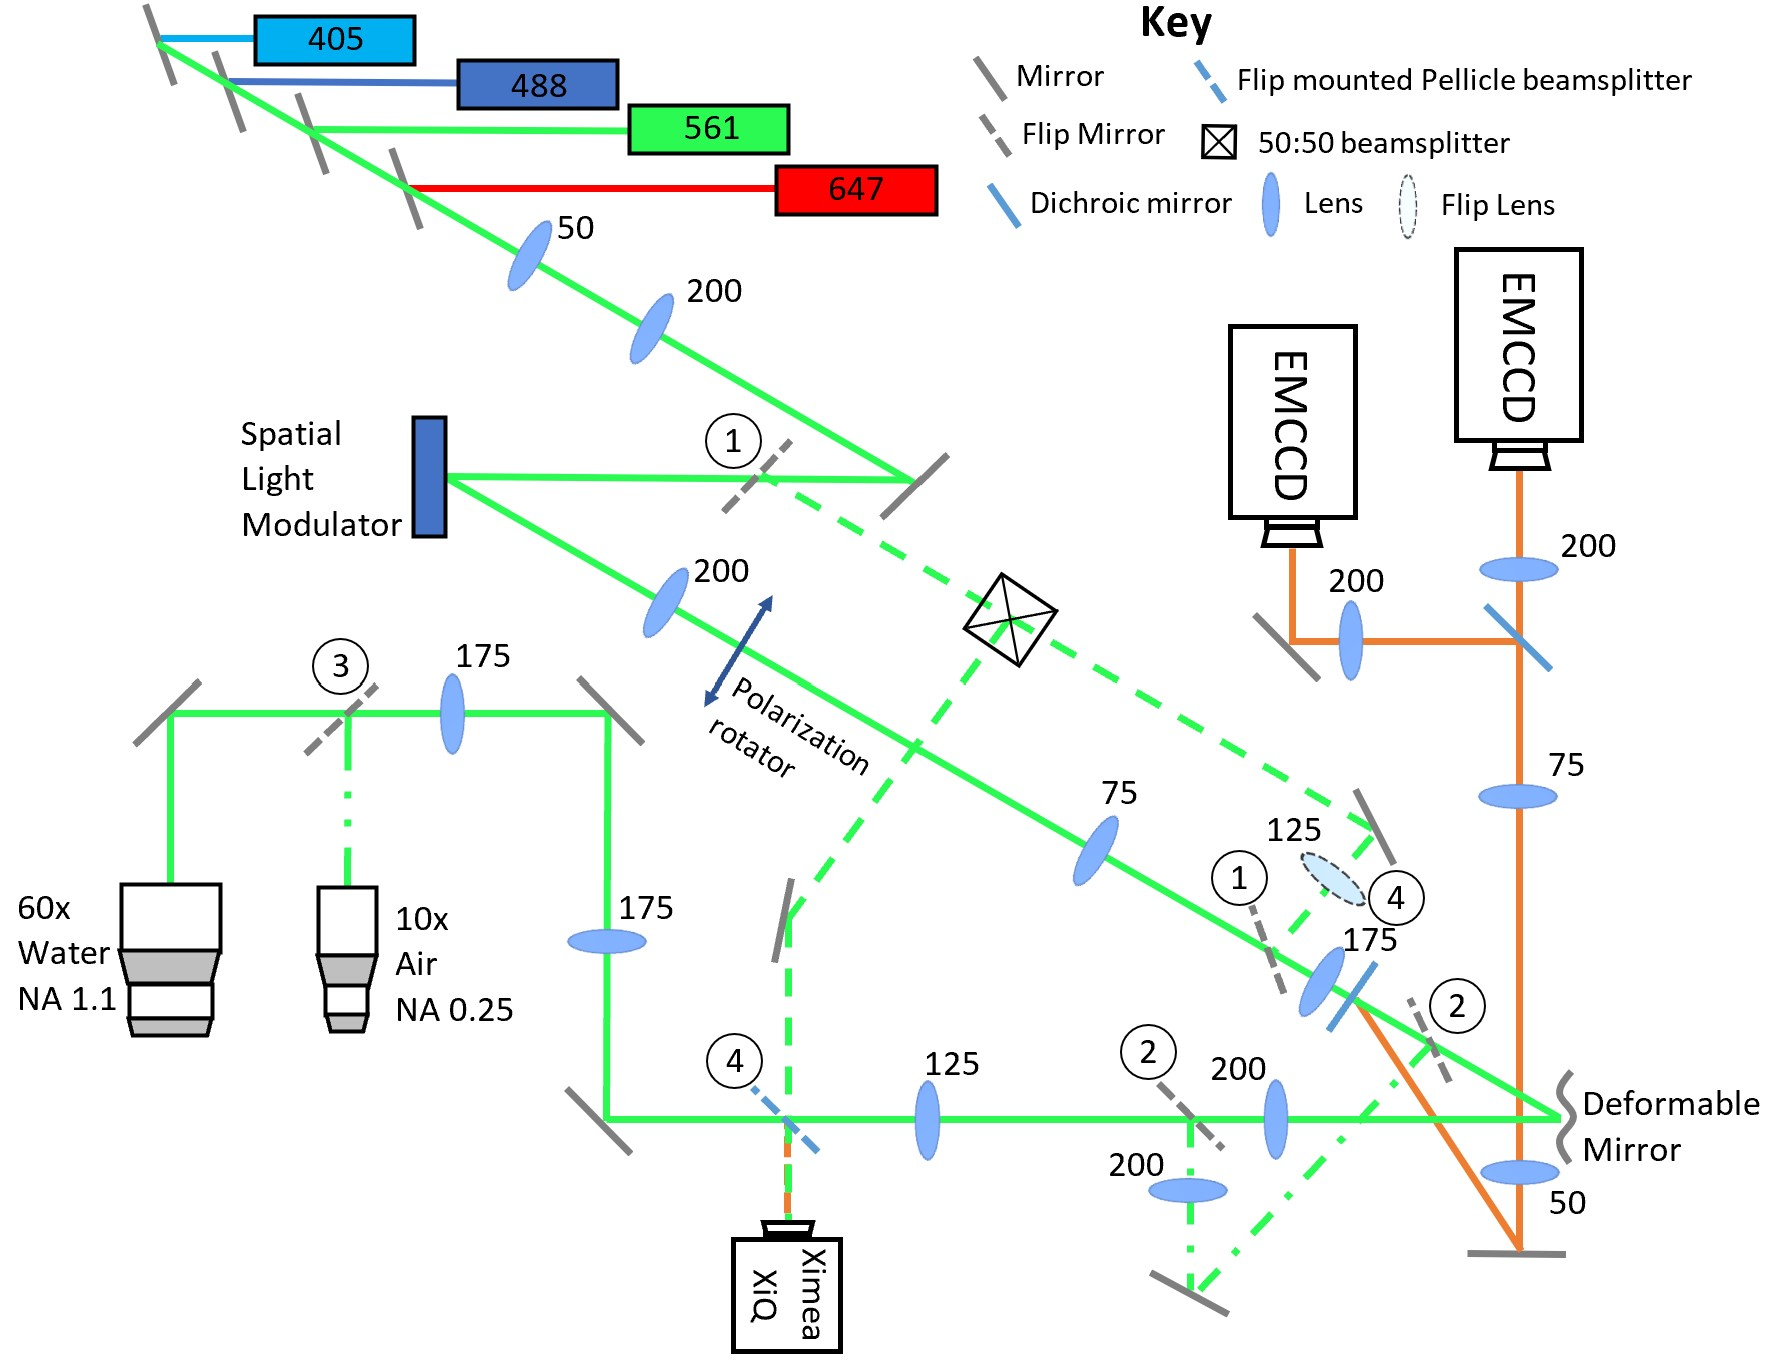
\includegraphics[width=\textwidth]{images/DeepSIM_complete_beam_paths.jpg}
	\caption{Complete beam path layout for DeepSIM. DeepSIM has multiple paths that can be selected by flipping the numbered pairs/individual mirrors. The green paths denotes the excitation beam paths. The solid green path shows the structured illumination (SI) beam path. The dashed green path shows the widefield beam path. This is changed to the interference beam path by flipping up the lens and pellicle pair. The dot-dashed green path shows the excitation path which bypasses the deformable mirror. The dot-dot-dashed green path shows the excitation path going through the $10\times$ air objective for low magnification sample mapping. The orange path denotes the emission beam path.}
	\label{fig:DeepSIM_complete_beam_paths}
\end{figure}

Raising the \circled{1} pair of flip mirrors bypasses the SLM and changes the excitation beam path to a widefield configuration. Raising the \circled{2} pair of flip mirrors bypasses the DM. This is a useful configuration when the DM has not yet been calibrated since the neutral position of the DM actuators have a worse flatness profile than that of a plane mirror. Without calibration, the DM surface cannot be flattened and may contribute to the aberrations present in the imaging system. Raising the \circled{3} flip mirror directs the excitation beam path through the $10 \times$ air objective. This beam path is used for large field of view (FOV) mapping.

Raising both the \circled{1} pair of flip mirrors and the \circled{4} flip mounted pellicle beamsplitter and lens changes both the excitation and emission beam paths to create an interferometer. Half of the excitation beam is picked off by the 50:50 beamsplitter and directed straight into the Ximea XiQ camera. This is the interferometer reference arm. The sample beam arm proceeds through the regular excitation beam path. Placing a mirror in the focal plane of the $60\times$ objective reflects the beam back through the emission beam path until it is reflected by the pellicle into the Ximea XiQ camera. The interference pattern produce by the two beams can interrogated to yield an image of the wavefront phase. Since the DM is in the sample arm, varying the shape of the DM surface will change the shape of the phase wavefront. Measuring how the movement of the DM's actuators influences the shape of the phase wavefront allows the DM to be calibrated and subsequently used to correct for aberrations in the optical system or sample. 

\subsection{Optical Alignment}
\label{subsec:alignment}

Being a bespoke microscopy system, DeepSIM was assembled from individual components and aligned by hand. This alignment process is critical for ensuring the microscopy system itself introduces the smallest possible aberrations. Aberrations in the imaging system disrupt image formation and degrade image quality.\cite{wyant1992basic} This affects both the excitation and emission paths of any fluorescent microscope. For a SIM microscope such as DeepSIM the most noticeable effect in the excitation path is the degradation of the structured illumination pattern, particularly the high frequency components.\cite{debarre2008adaptive,booth2015aberrations} In the emission path, these aberrations prevent correct image formation on the cameras sensors. Whilst DeepSIM incorporates a DM for performing aberration correction, every DM has a limited stroke length and the actuator response is often non-linear at the limits of this stroke length. Correcting for relatively large system aberrations due to a poorly aligned system is likely to lead to insufficient remaining stroke length to correct for sample induced aberrations. Therefore, having a well aligned system is still critical even for AO-enabled microscopy systems such as DeepSIM.

Firstly the upright bridge to hold the objectives and the stage in their upright configuration was constructed and installed on the optical table. One of the lasers was then installed and the beam paths shown in Figure~\ref{fig:DeepSIM_complete_beam_paths} was constructed without the lenses. The beam was kept either parallel or perpendicular to the optical table where appropriate and passing through the centre of the objective aperture. The beam was kept parallel to the table by positioning an iris at the beam height at the laser and 'walking' this iris down the beam path, ensuring that after each reflection the beam remains at the same height. Once this beam path was established, the lenses were added sequentially and aligned. Finally, the other lasers are coaligned to this beam path. The result is the complete optical setup shown in Figure~\ref{fig:DeepSIM_physical_optics}.

\begin{figure}[h]
	\centering
	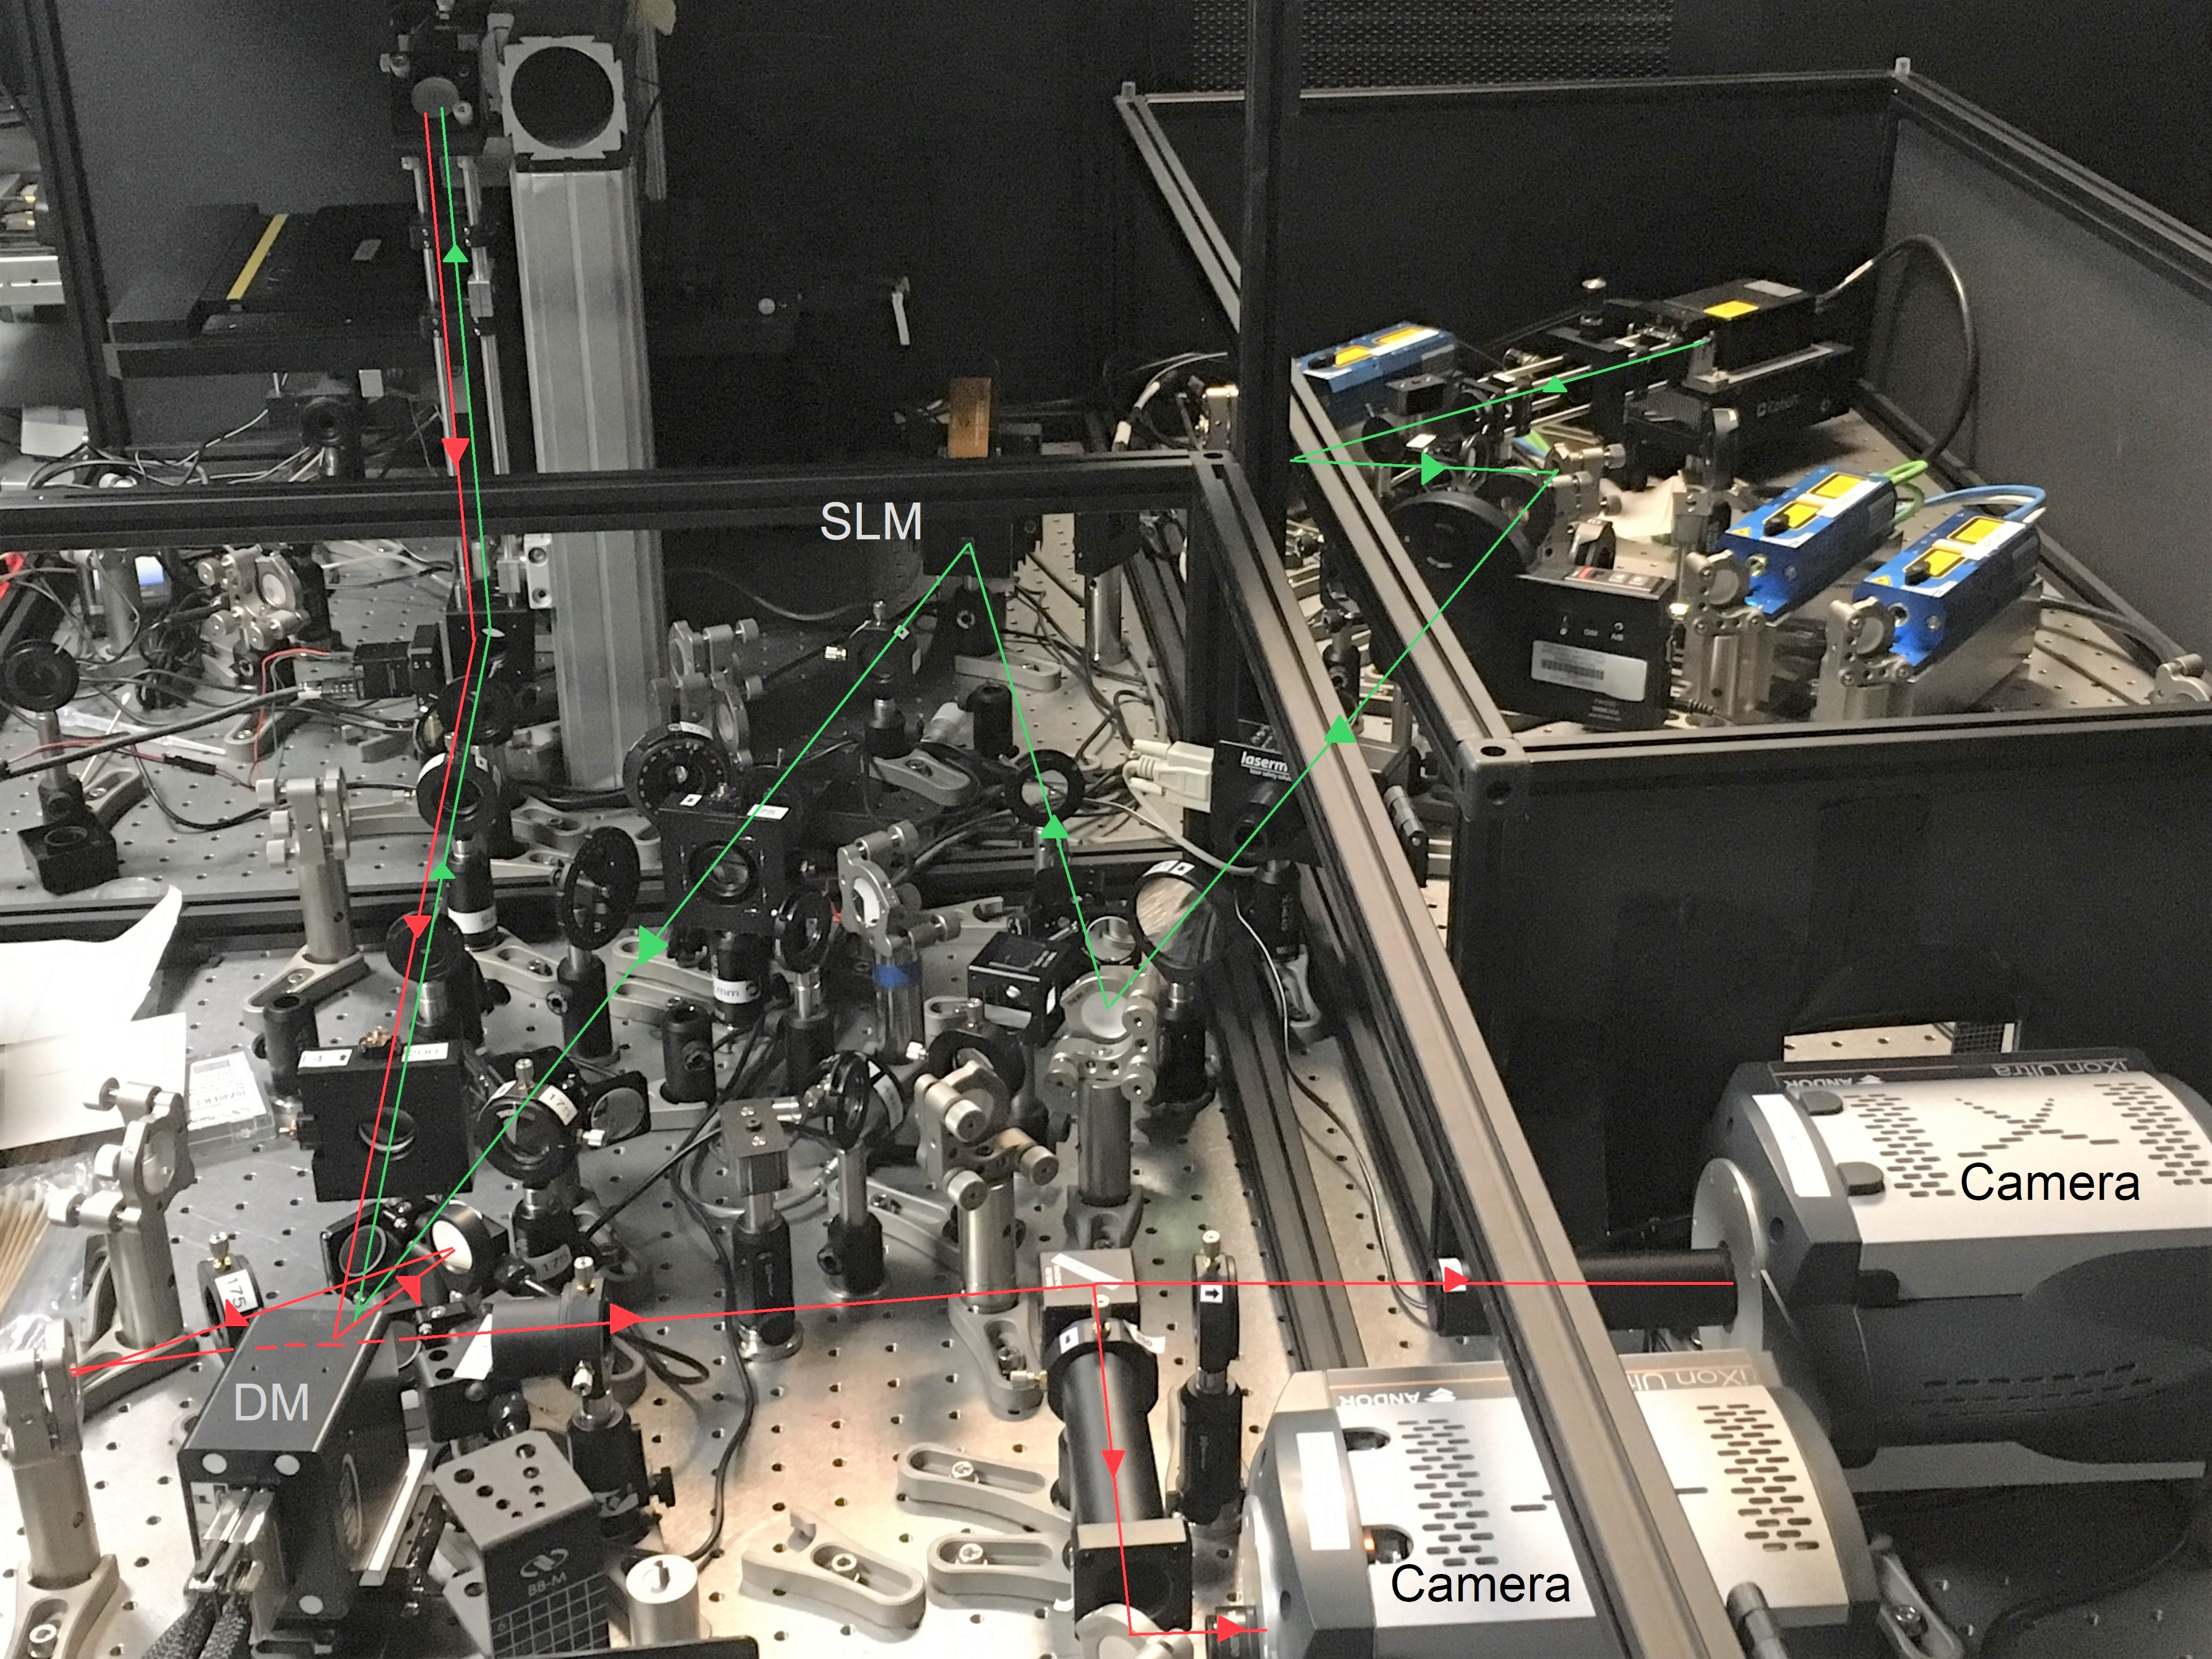
\includegraphics[width=\textwidth]{images/DeepSIM_SIM_path_annotated_bright.jpg}
	\caption{The aligned DeepSIM optical set-up. The 3D-SIM excitation (green) and emission (red) beam paths are annotated.}
	\label{fig:DeepSIM_physical_optics}
\end{figure}

The alignment of the lenses and the coalignment of the lasers is typically done by eye. The quality of the alignment done in this manner is highly subjective and dependant on a number of factors that affect the quality of the operators judgement that two beams are in the same position on an pinhole/iris. BeamDelta was used to align the optical components of DeepSIM as it offers a more accurate, less hazardous and faster approach to optical element alignment.\cite{dobbie2019beamdelta}

\section{Control Software}
\label{sec:control_software}

\subsection{\textit{Python Microscope}}
\label{subsec:microscope}

There is a requirement for control over all the hardware elements of an optical system. This can pose a problem since each hardware component has its own low level software libraries and the physical hardware is connected to several different computers. Additionally, in order to ensure rapid imaging of 3D widefield and SIM Z-data stacks there is a requirement for precise timing control of the electronic hardware, such as laser, cameras, etc, which must act in concert. To solve these challenges, hardware on both the Aurox Clarity and DeepSIM systems are controlled via Python Microscope, an open source Python package which allows the various elements to be synchronised with hardware triggers. For this, a RedPitaya is used on each system and functions as a digital signal processor (DSP).

\subsection{\textit{Microscope-Cockpit}}
\label{subsec:cockpit}

Optical systems require a bespoke graphical user interface (GUI) which is accessible to users. For this purpose Cockpit, highly flexible and adaptable open source Python-base GUI environment, is utilised for both systems. Figure~\ref{fig:Cockpit_UI} shows the GUI used to control DeepSIM. In the main window, Figure~\ref{fig:DeepSIM_control_software_main_window}, a user can enable and disable the various hardware elements. They can also swap between the various beam paths shown in Figure~\ref{fig:DeepSIM_complete_beam_paths}. A user also has access to the automated AO methods, the specifics of which will be discussed later. Figure~\ref{fig:DeepSIM_control_software_stage_control} shows the window which can be used to control the XY stage, and the coarse mechanical and fine piezo Z stages as well as display the location of each. The step control and step size for each of these are assigned to keyboard shortcuts. 

\begin{figure}[h]
	\centering
	\begin{subfigure}{0.575\textwidth}
		\centering
		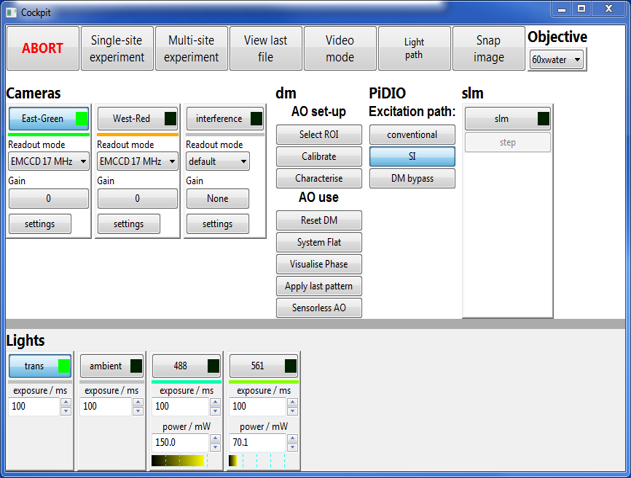
\includegraphics[width=\linewidth]{images/DeepSIM_control_software_main_window.png}
		\caption{}
		\label{fig:DeepSIM_control_software_main_window}
	\end{subfigure}
	\begin{subfigure}{0.365\textwidth}
		\centering
		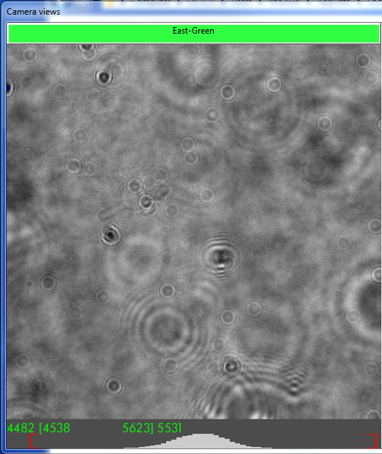
\includegraphics[width=\linewidth]{images/DeepSIM_control_software_camera.png}
		\caption{}
		\label{fig:DeepSIM_control_software_camera}
	\end{subfigure}
	
	\begin{subfigure}{0.51\textwidth}
		\centering
		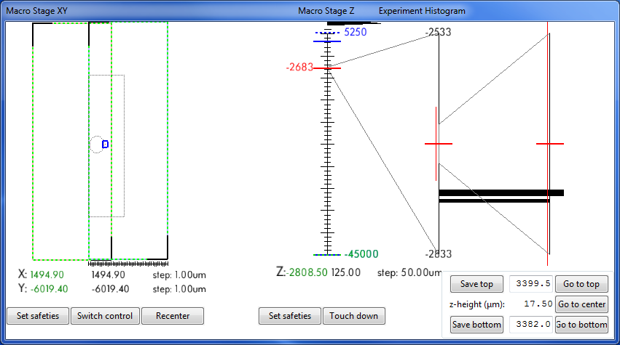
\includegraphics[width=\linewidth]{images/DeepSIM_control_software_stage_control.png}
		\caption{}
		\label{fig:DeepSIM_control_software_stage_control}
	\end{subfigure}
	\begin{subfigure}{0.45\textwidth}
		\centering
		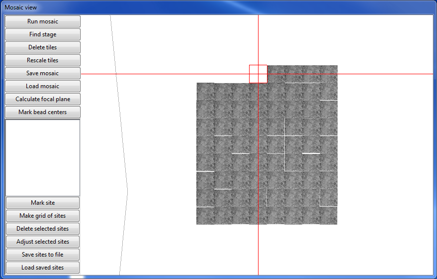
\includegraphics[width=\linewidth]{images/DeepSIM_control_software_mosaic.png}
		\caption{}
		\label{fig:DeepSIM_control_software_mosaic}
	\end{subfigure}
	\caption{Cockpit GUI for controlling DeepSIM (a) Cockpit main window. Contains buttons to enable all the hardware, set laser powers and change beam paths (b) Camera view window. Shows the most recent readout from all the enabled cameras (c) Stage control window. Allows the user to control the position of the XY piezo-stage, coarse mechanical Z stage and fine Z piezo-stage (d) Mosaic window. Used by the user to scan the field of view for structures of interest and mark them.}
	\label{fig:Cockpit_UI}
\end{figure}

Unlike commercial microscopes, DeepSIM does not have any eye-pieces. Ordinarily this would present a problem for simply locating the sample, let alone locating a specific region or structure of interest within the sample. To overcome this limitation, Cockpit implements a Mosaic window shown in Figure~\ref{fig:DeepSIM_control_software_mosaic}. When the mosaic is run, Cockpit moves the stage in a anti-clockwise spiral pattern and takes an image at each position. These images are stored on the main machine's graphics card to enable real-time navigation and site-of-interest marking. Since the images are stored, a user can revisit and investigate areas of the sample which have already been imaged without re-imaging them, decreasing the light exposure and limiting photodamage. The user is able to take an initial mosaic using the $10\times$ objective to find the sample, create a specimen guide map and identify regions of interest. They then swap to the $60\times$ objective for a more detailed mosaic in the previously identified regions, locate specific sites of interest which they can then mark. These sites can then be visited by the user individually and have data collected manually using the "Single-site experiment" option or each site can be visited and data collected in an automated fashion using the "Multi-site experiment option". In this way DeepSIM can function well without eye-pieces and is easily controlled by a potential user.
